% !TEX root = ../../main.tex
\section{Data Gathering}\label{sec:data_gathering}
For our data sets of real world activities we have sampled both in- and outdoor activities.
The subjects performing the activities are three males, in an age around 25.
We have used two series of recordings.
The first series are various outdoor recordings with segments of walking, running and standing.
Some movement activities are performed in a straight line, whilst others are performed around corners of in a wide circular direction.
The second series consist of mainly walking up and down the stairs, with small vertical parts between the segments.
The stairs are all in a circular shape.

\subsection{Outdoor straight lines}\label{subsec:outdoor_straight}
The first series of outdoor performed activities consist of walking and running segments in a straight line.
Halfway the recording is a $180^{\circ}$ turn.
The activities consist of standing still, walking and running (both jogging and sprinting).
The plots of \Cref{fig:data_gathering_run_1_rot,fig:data_gathering_run_1_acc,fig:data_gathering_run_1_mag} shows the recordings of Subject $1$.
For Subject $2$ the plots are visible in \Cref{fig:data_gathering_run_2_rot,fig:data_gathering_run_2_acc,fig:data_gathering_run_2_mag}.
The recorded metrics are from the accelerometer, rotational and magnetometer sensors.
The solid black lines indicate manually annoted change points, the dashes lines indicate the closest discovered change point.
A still from the video recording, showing Subject $2$ performing a (sprinting) run segment, is in \Cref{fig:data_gathering_still_1_sprint}.

\TODO{Add found change points to plots}

%---- Run 1: walk-run-roemer
\begin{figure}
\centering
  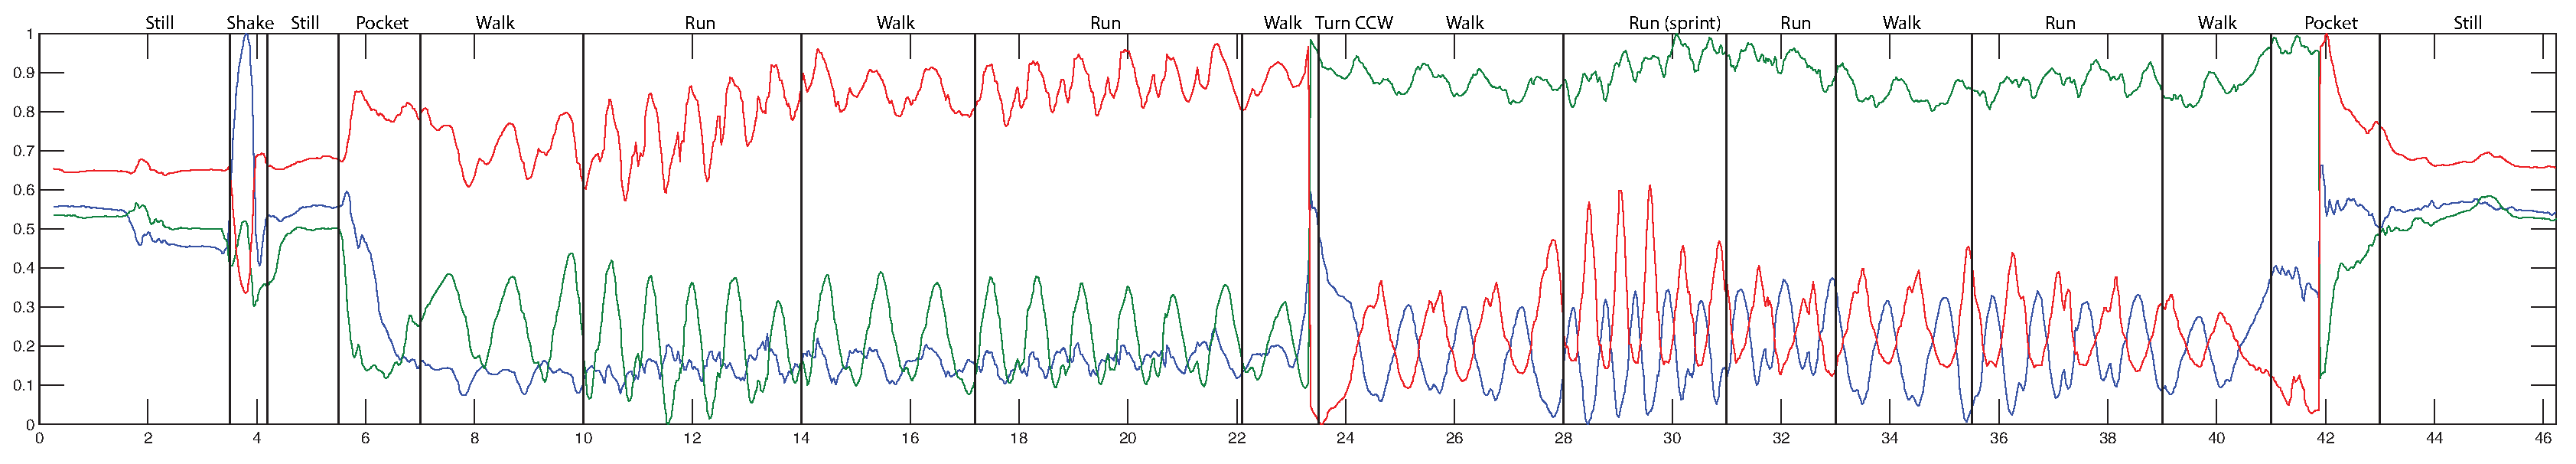
\includegraphics[width=1\textwidth]{./Figures/chapter6/data_collection/run-1-walk-run-roemer/data_plot_rot_annotated.eps}
  \caption[R1: rotation]{Run 1: Walk-run-roemer, rotation}
  \label{fig:data_gathering_run_1_rot}
\end{figure}

\begin{figure}
\centering
  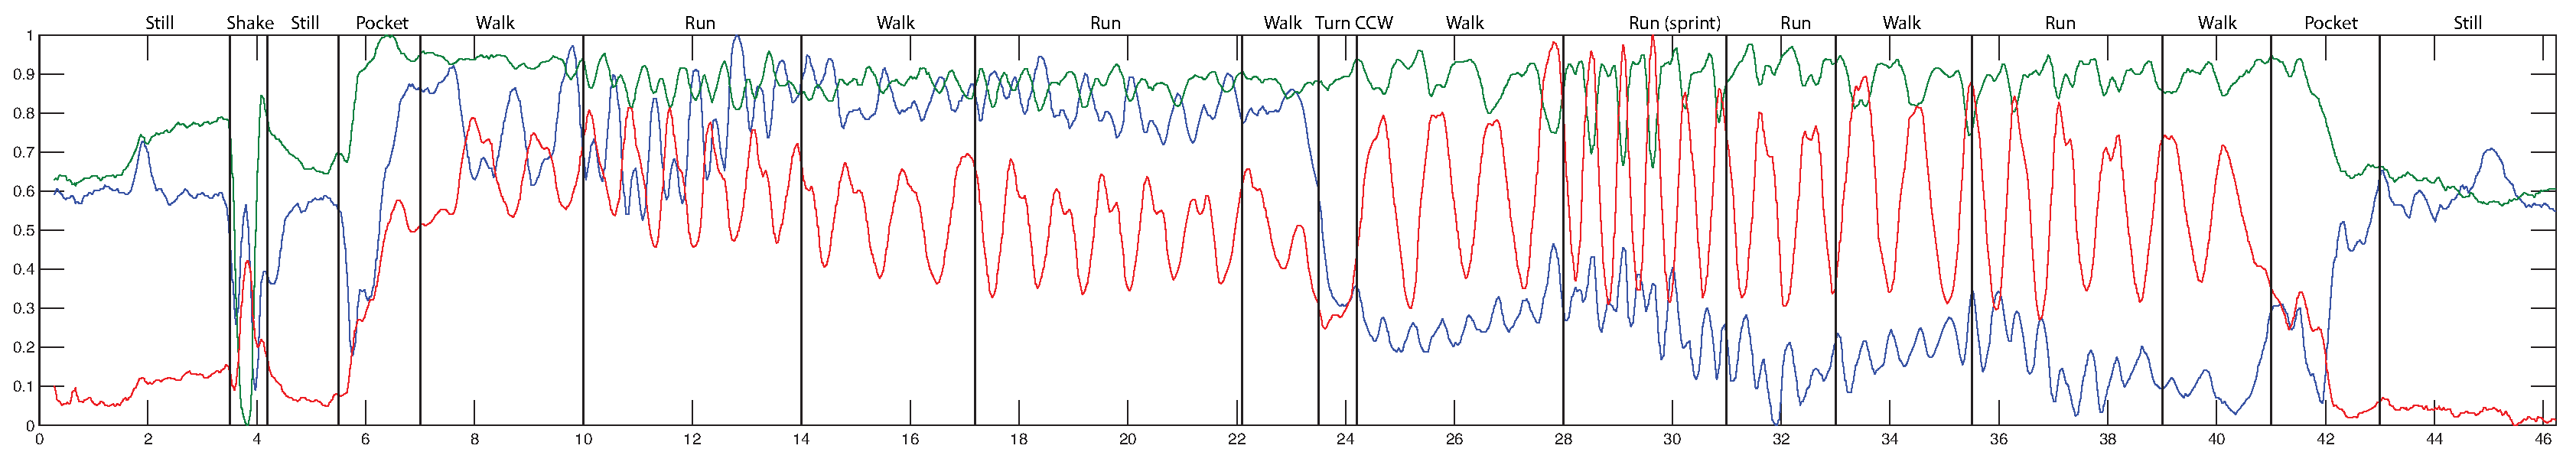
\includegraphics[width=1\textwidth]{./Figures/chapter6/data_collection/run-1-walk-run-roemer/data_plot_mag_annotated.eps}
  \caption[R1: mag]{Run 1: Walk-run-roemer, Mag}
  \label{fig:data_gathering_run_1_mag}
\end{figure}

\begin{figure}
\centering
  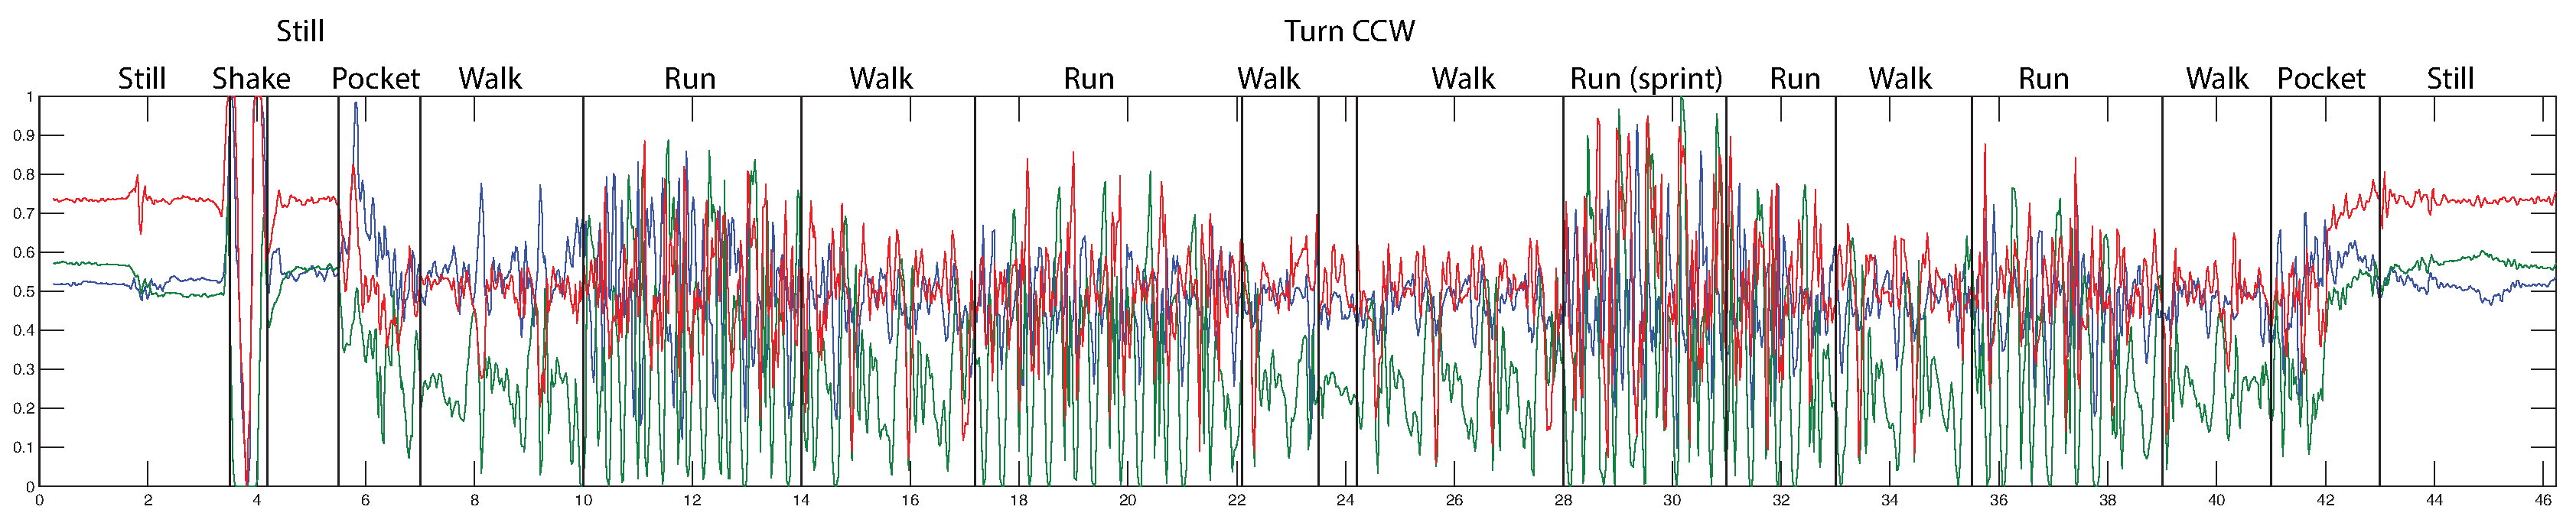
\includegraphics[width=1\textwidth]{./Figures/chapter6/data_collection/run-1-walk-run-roemer/data_plot_acc_annotated.eps}
  \caption[R1: accelerometer]{Run 1: Walk-run-roemer, accelerometer}
  \label{fig:data_gathering_run_1_acc}
\end{figure}

%---- Run 2: walk-run-jos
\begin{figure}
\centering
  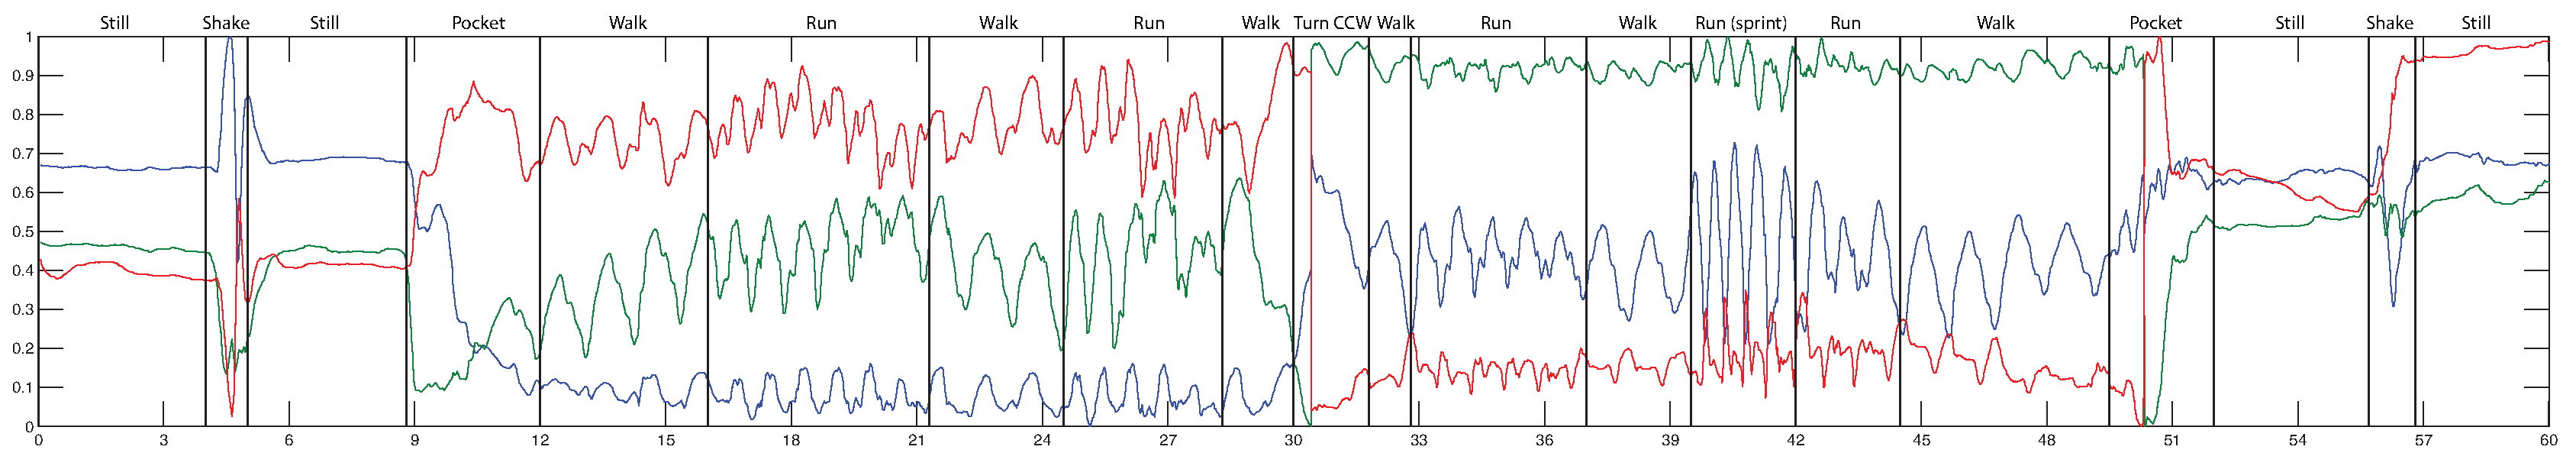
\includegraphics[width=1\textwidth]{./Figures/chapter6/data_collection/run-2-walk-run-jos/data_plot_rot_annotated.eps}
  \caption[R2: rotation]{Run 2: Walk-run-jos, rotation}
  \label{fig:data_gathering_run_2_rot}
\end{figure}

\begin{figure}
\centering
  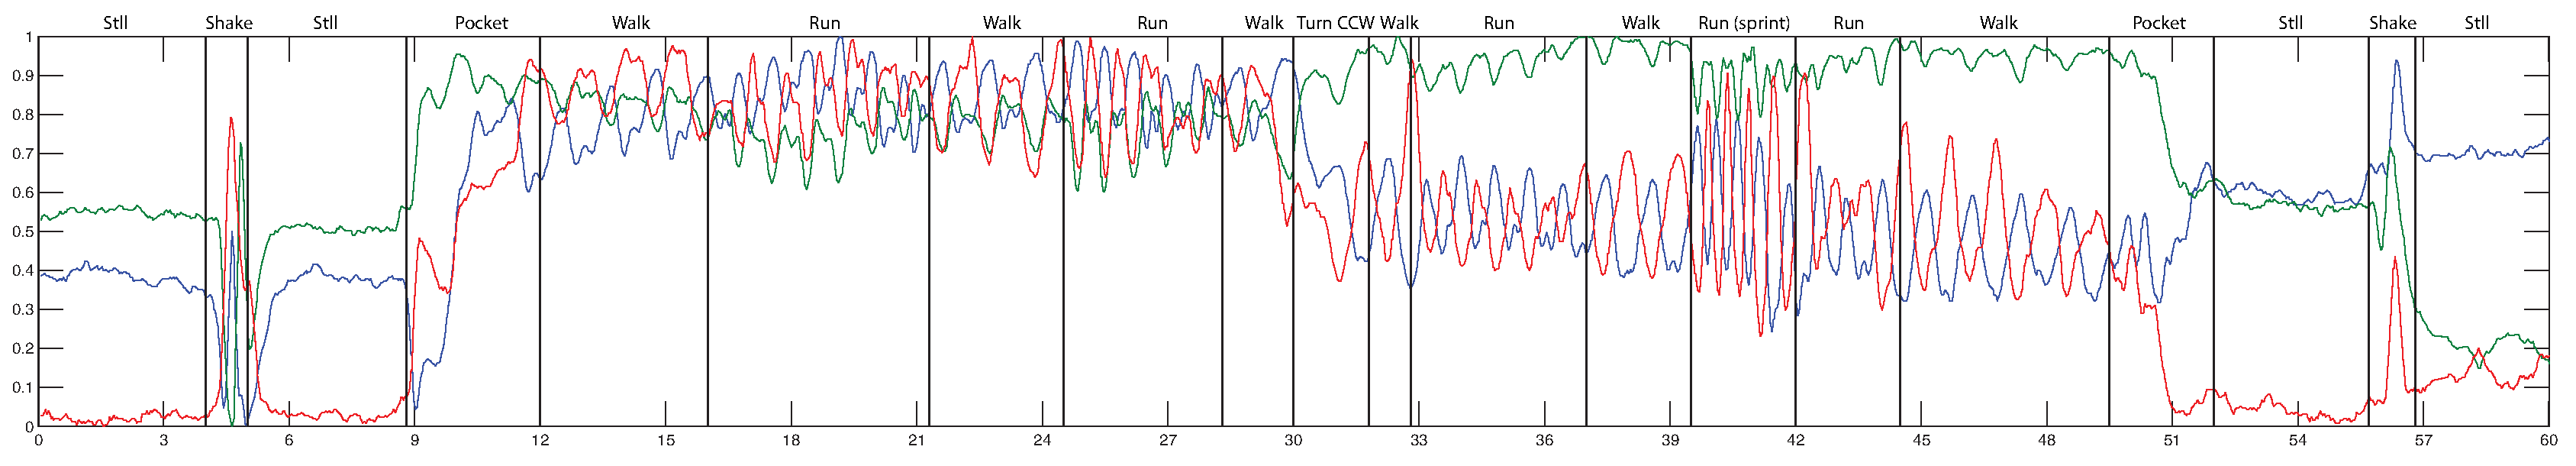
\includegraphics[width=1\textwidth]{./Figures/chapter6/data_collection/run-2-walk-run-jos/data_plot_mag_annotated.eps}
  \caption[R2: mag]{Run 2: Walk-run-jos, Mag}
  \label{fig:data_gathering_run_2_mag}
\end{figure}

\begin{figure}
\centering
  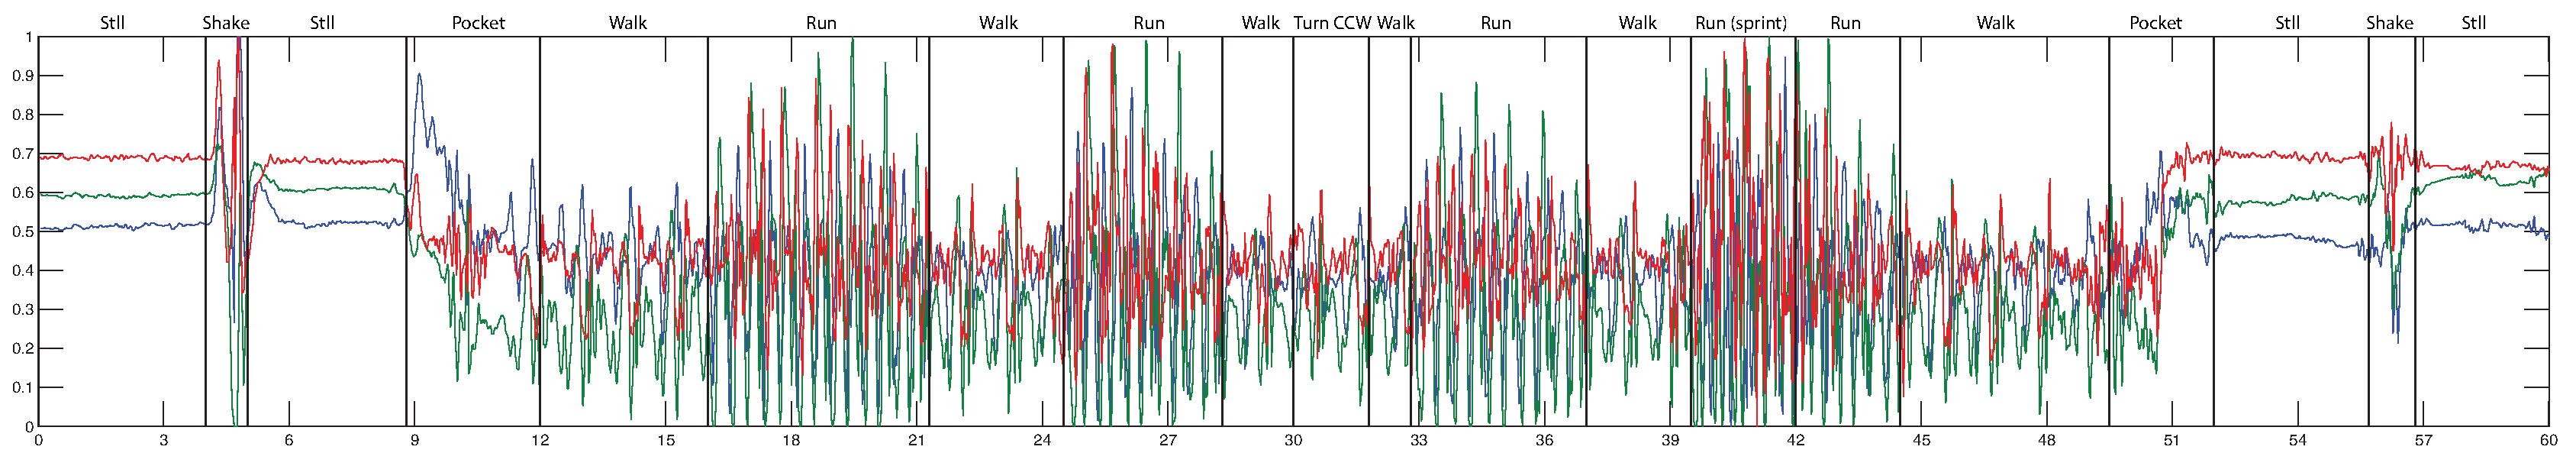
\includegraphics[width=1\textwidth]{./Figures/chapter6/data_collection/run-2-walk-run-jos/data_plot_acc_annotated.eps}
  \caption[R2: accelerometer]{Run 2: Walk-run-jos, accelerometer}
  \label{fig:data_gathering_run_2_acc}
\end{figure}


%=== STILLS
\begin{figure}
\centering
  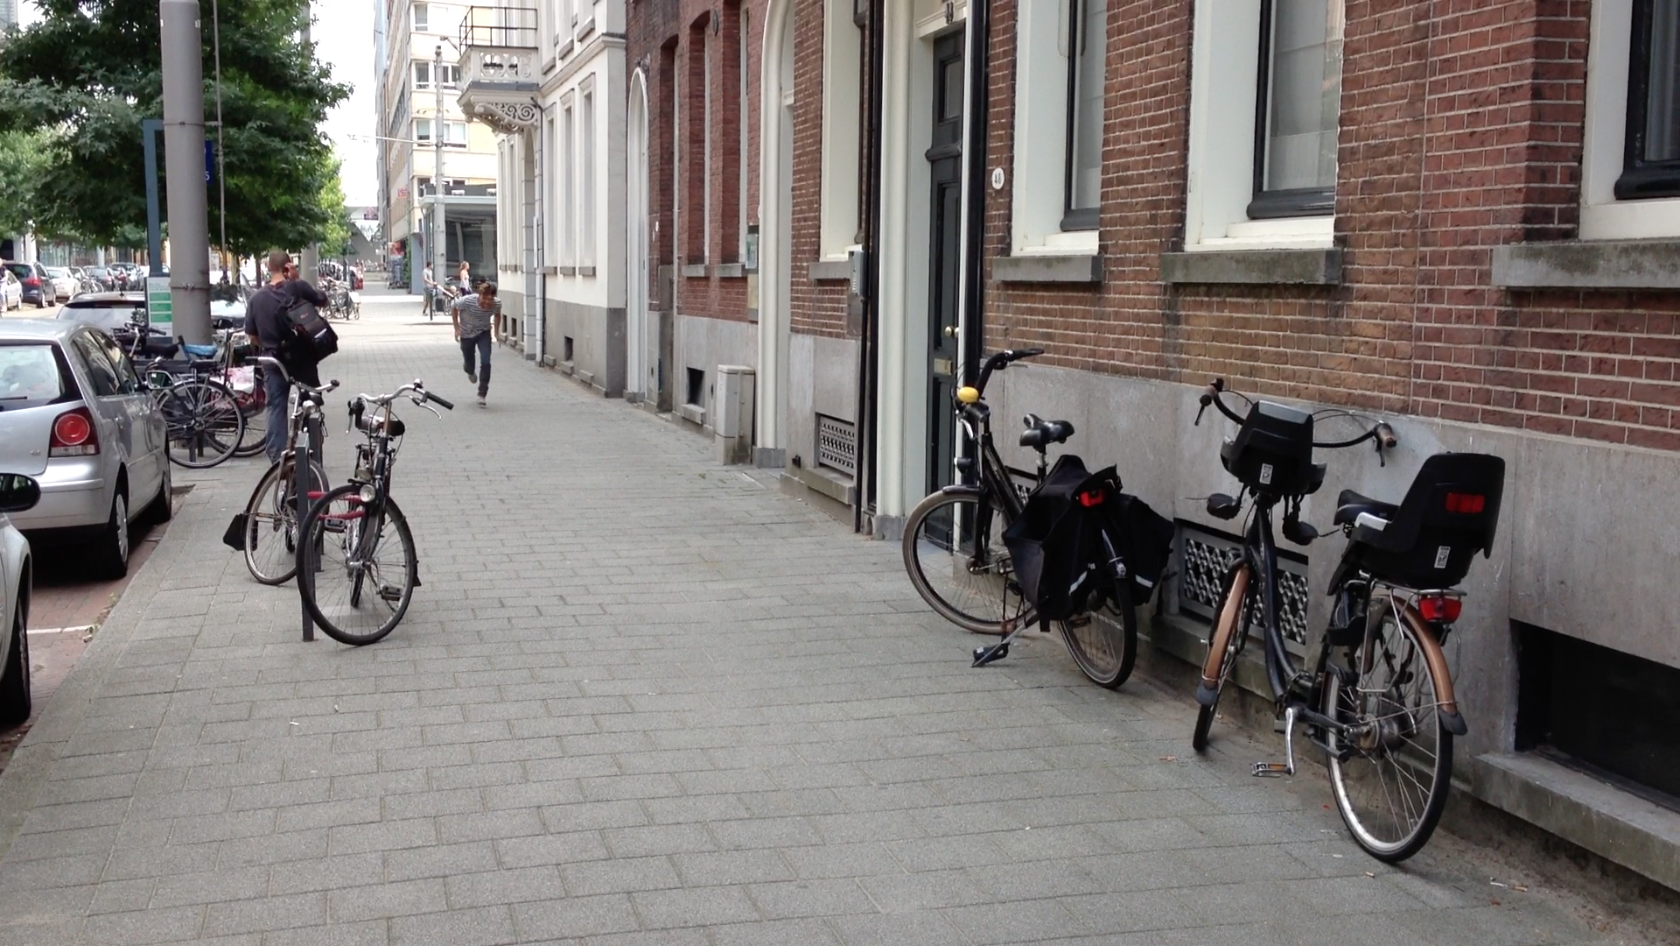
\includegraphics[width=1\textwidth]{./Figures/chapter6/data_collection/stills/jos_sprint.png}
  \caption[Recording still 4]{Subject 1 sprinting}
  \label{fig:data_gathering_still_1_sprint}
\end{figure}





\subsection{Outdoor straight lines results}
\TODO{For each data set: discovered timepoint with acc, mag, rot, and all combined. Use closest change point}

\begin{center}\begin{table}
  \begin{tabulary}{\textwidth}{|l|c|c|}
    \hline
    \multicolumn{3}{|c|}{Subj 1, run 1} \\
    \hline \hline
    Act. & Ann. & Disc. \\
    \hline
    Still & 0 & *0* \\
    \hline
    Shake & 3.5 & *3.5* \\
    \hline
    Still & 4.2 & *4.2* \\
    \hline
    In pocket & 5.5 & *5.5* \\
    \hline
    Walk & 7 & *7* \\
    \hline
    Run & 10 & *10* \\
    \hline
    Walk & 14 & *14* \\
    \hline
    Run & 17.2 & *17.2* \\
    \hline
    Walk & 22.1 & *22.1* \\
    \hline
    Turn CCW & 23.5 & *23.5* \\
    \hline
    Walk & 24.2 & *24.2* \\
    \hline
    Run (sprint) & 28 & *28* \\
    \hline
    Run & 31 & *31* \\
    \hline
    Walk & 33 & *33* \\
    \hline
    Run & 35.5 & *35.5* \\
    \hline
    Walk & 39 & *39* \\
    \hline
    Out pocket & 41 & *41* \\
    \hline
    Still & 43 & *43* \\
    \hline
    \hline
    \multicolumn{2}{|l|}{Ratio Total CPs} & 3.2 \\
    \hline
    \multicolumn{2}{|l|}{Sum of differences} & 12.341 \\
    \hline
  \end{tabulary}
  \caption[Performed activities subject 1 run 1]{The outdoor series performed activities by subject 1, run 1.}
  \label{tab:outdoor_series}
\end{table}\end{center}

\TODO{Replace all times in the stars with the closest discovered change point}

% ===== OUTDOOR FREE ACTIVITIES ========
\subsection{Outdoor free}\label{subsec:outdoor_free}
The second series of outdoor recordings consist of more free-form activities.
The performed activities consist, as with the first set, of standing, walking, and running.
Furthermore, the segments are performed in a circular manner.
\eg the running activities are performed around a fountain with an estimated diameter of 10 meters.
The plots of the recordings of Subject, for the accelerometer, rotation, and magnetometer are shown in...
\TODO{Add plots}
For Subject $2$ the still of the video recordings are in \Cref{fig:data_gathering_still_1_still_walk_to_run,fig:data_gathering_still_1_running,fig:data_gathering_still_1_running_2,fig:data_gathering_still_1_walk}.
The stills for Subject $1$ are in \Cref{fig:data_gathering_still_2_run,fig:data_gathering_still_2_walk}.


\begin{figure}
\centering
  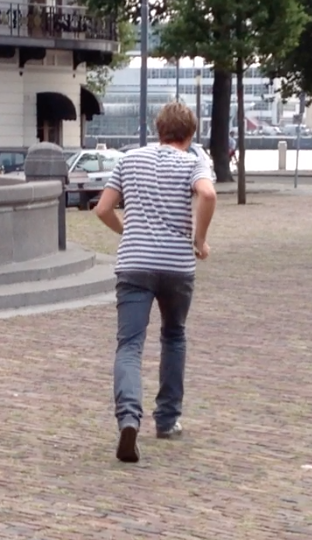
\includegraphics[width=1\textwidth]{./Figures/chapter6/data_collection/stills/jos_cp_walk-run.png}
  \caption[Recording still 1]{Subject 1 on the transition from walking to running}
  \label{fig:data_gathering_still_1_still_walk_to_run}
\end{figure}

\begin{figure}
\centering
  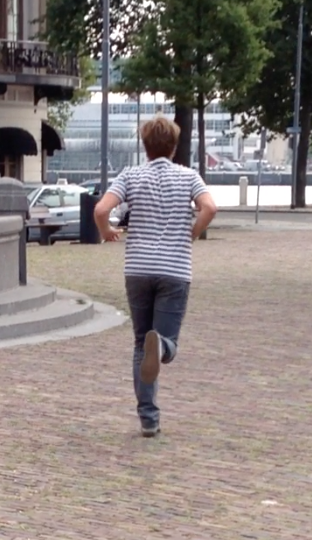
\includegraphics[width=1\textwidth]{./Figures/chapter6/data_collection/stills/jos_run_2.png}
  \caption[Recording still 2]{Subject 1 running}
  \label{fig:data_gathering_still_1_running}
\end{figure}

\begin{figure}
\centering
  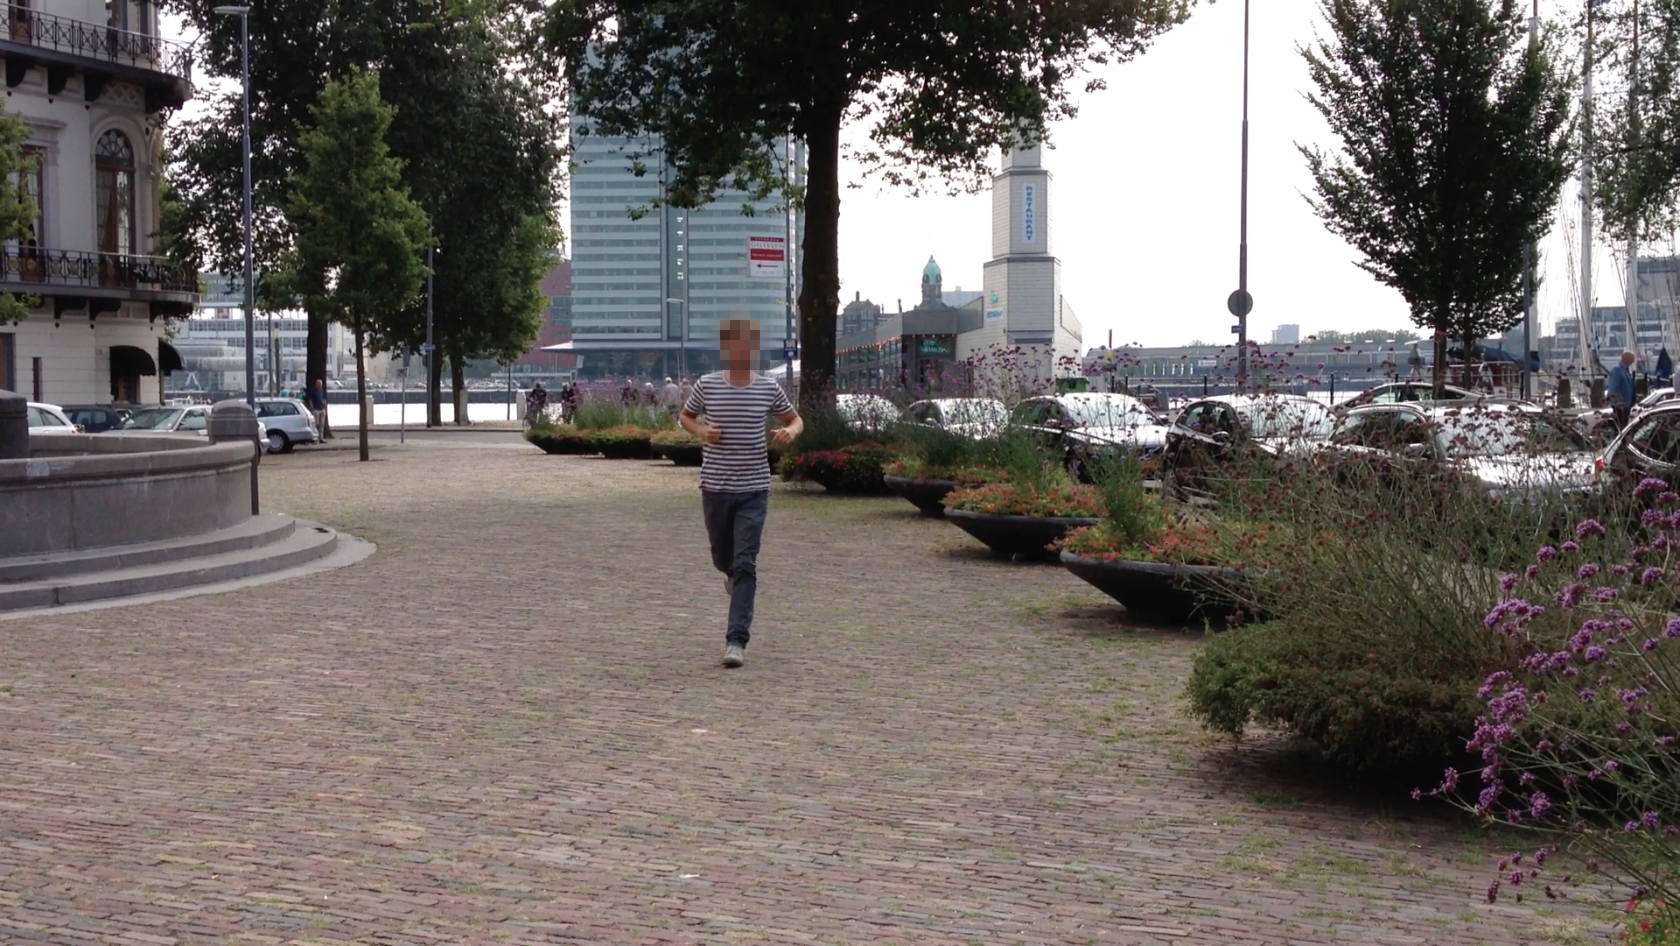
\includegraphics[width=1\textwidth]{./Figures/chapter6/data_collection/stills/jos_run.png}
  \caption[Recording still 3]{Subject 1 running}
  \label{fig:data_gathering_still_1_running_2}
\end{figure}

\begin{figure}
\centering
  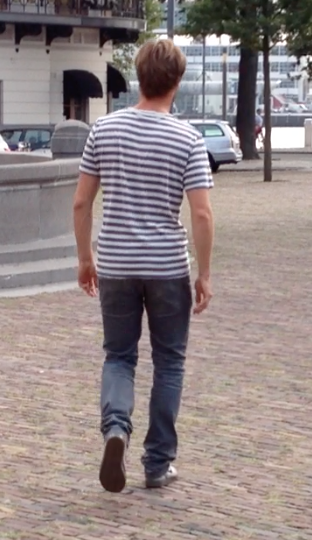
\includegraphics[width=1\textwidth]{./Figures/chapter6/data_collection/stills/jos_walking.png}
  \caption[Recording still 5]{Subject 1 walking}
  \label{fig:data_gathering_still_1_walk}
\end{figure}

Stills from subject 2:

\begin{figure}
\centering
  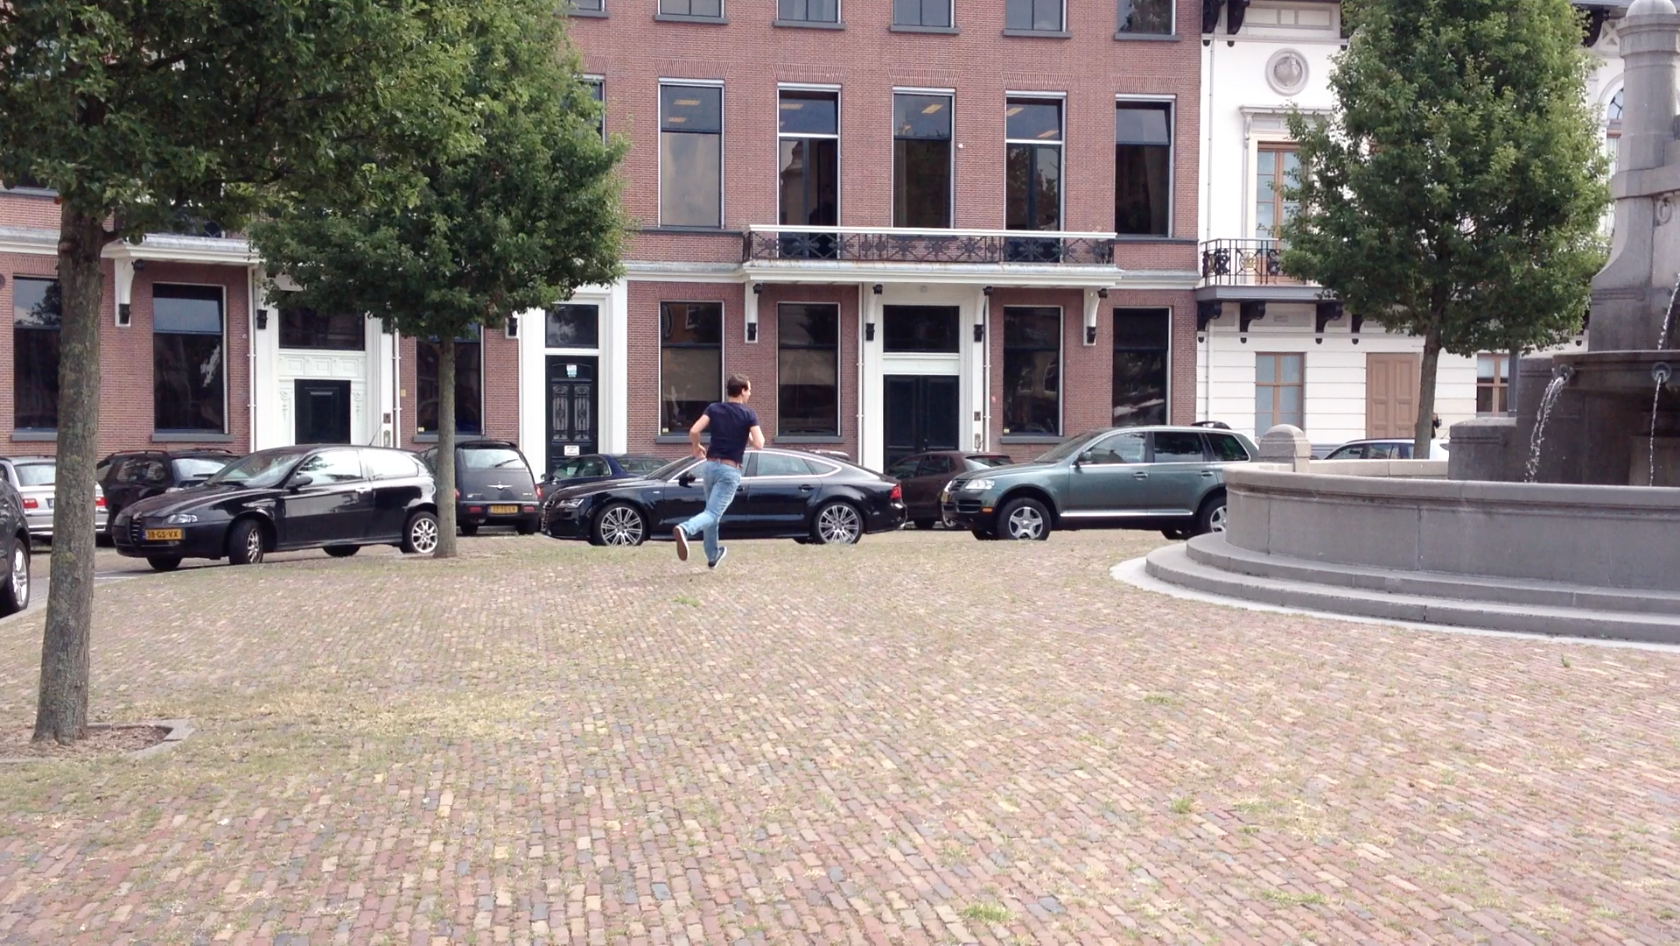
\includegraphics[width=1\textwidth]{./Figures/chapter6/data_collection/stills/roemer_run_cw.png}
  \caption[Recording still 6]{Subject 2 running in clockwise corner}
  \label{fig:data_gathering_still_2_run}
\end{figure}

\begin{figure}
\centering
  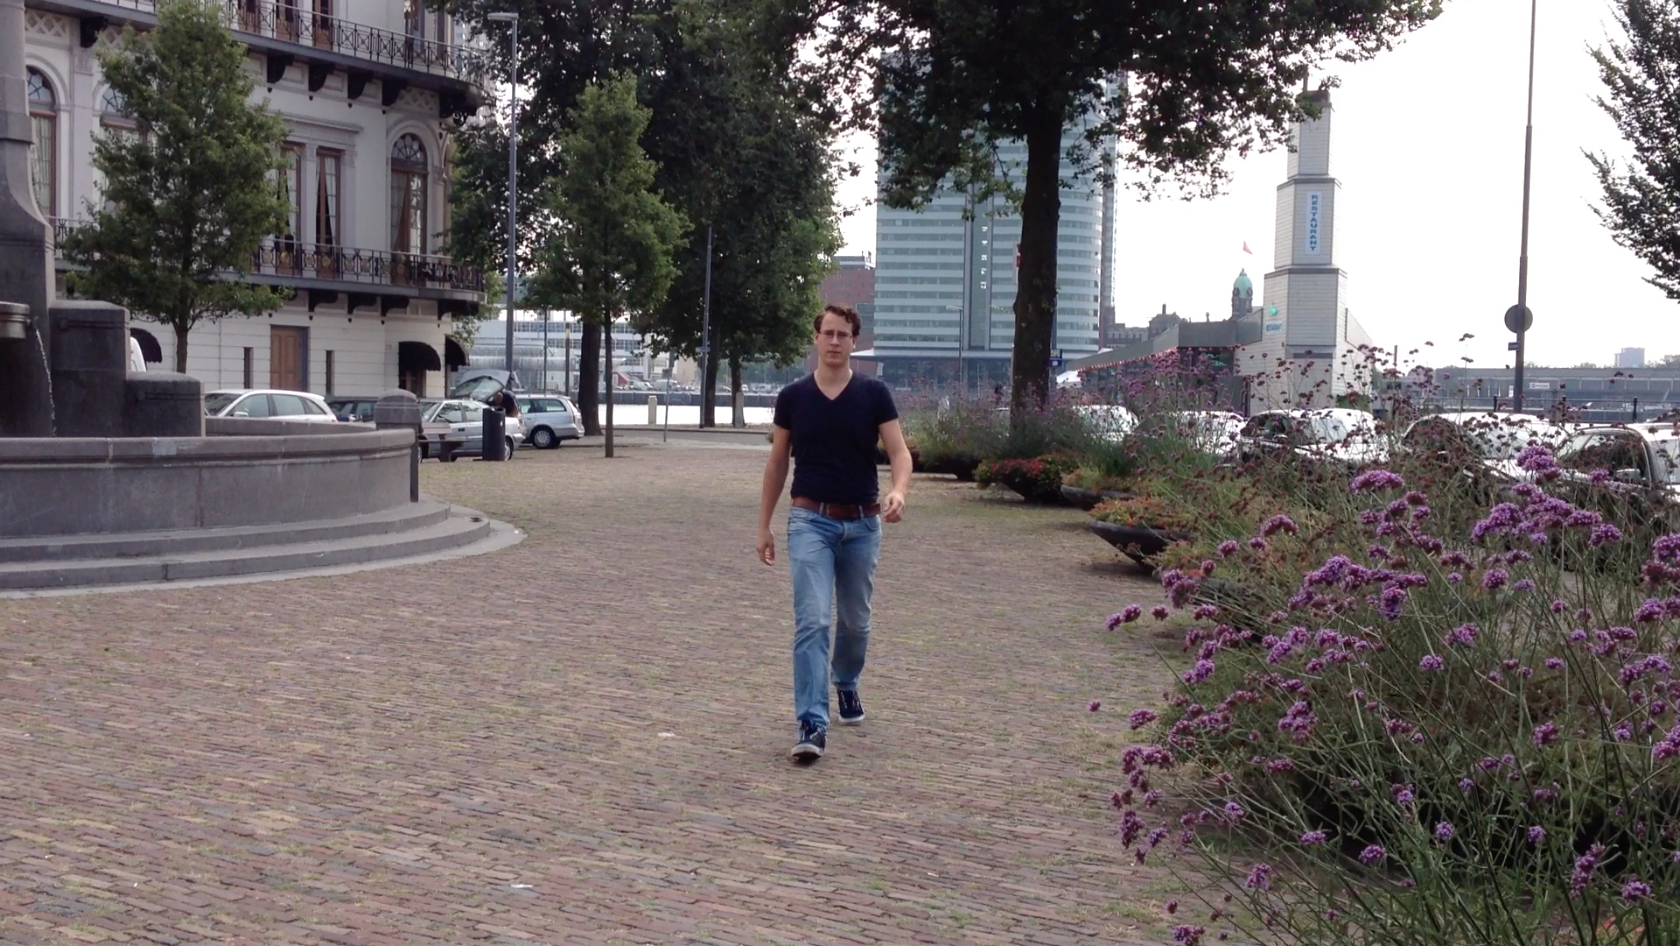
\includegraphics[width=1\textwidth]{./Figures/chapter6/data_collection/stills/roemer_walk.png}
  \caption[Recording still 7]{Subject 2 walking}
  \label{fig:data_gathering_still_2_walk}
\end{figure}



\subsection{Indoor stairs}\label{subsec:indoor_stairs}
The final series of activities recorded consist of walking up and down the stairs, indoor.
The stairs are shaped in an semi-circular form, with a small vertical segment on each floor.
The still of \Cref{fig:data_gathering_still_3_descending} illustrates the circular shape of the stairs.
In \Cref{fig:data_gathering_still_3_ascending} the small flat segment is visible.
Between the stairs the subject walked in a hallway with a $180^{\circ}$ counter-clockwise turn, as shown in \Cref{fig:data_gathering_still_3_walk}.
The recorded sensor data of the performed activities are visible in the plots of \Cref{fig:data_gathering_run_3_rot,fig:data_gathering_run_3_mag,fig:data_gathering_run_3_acc}.

%---- Run 3: Stairs remco
\begin{figure}
\centering
  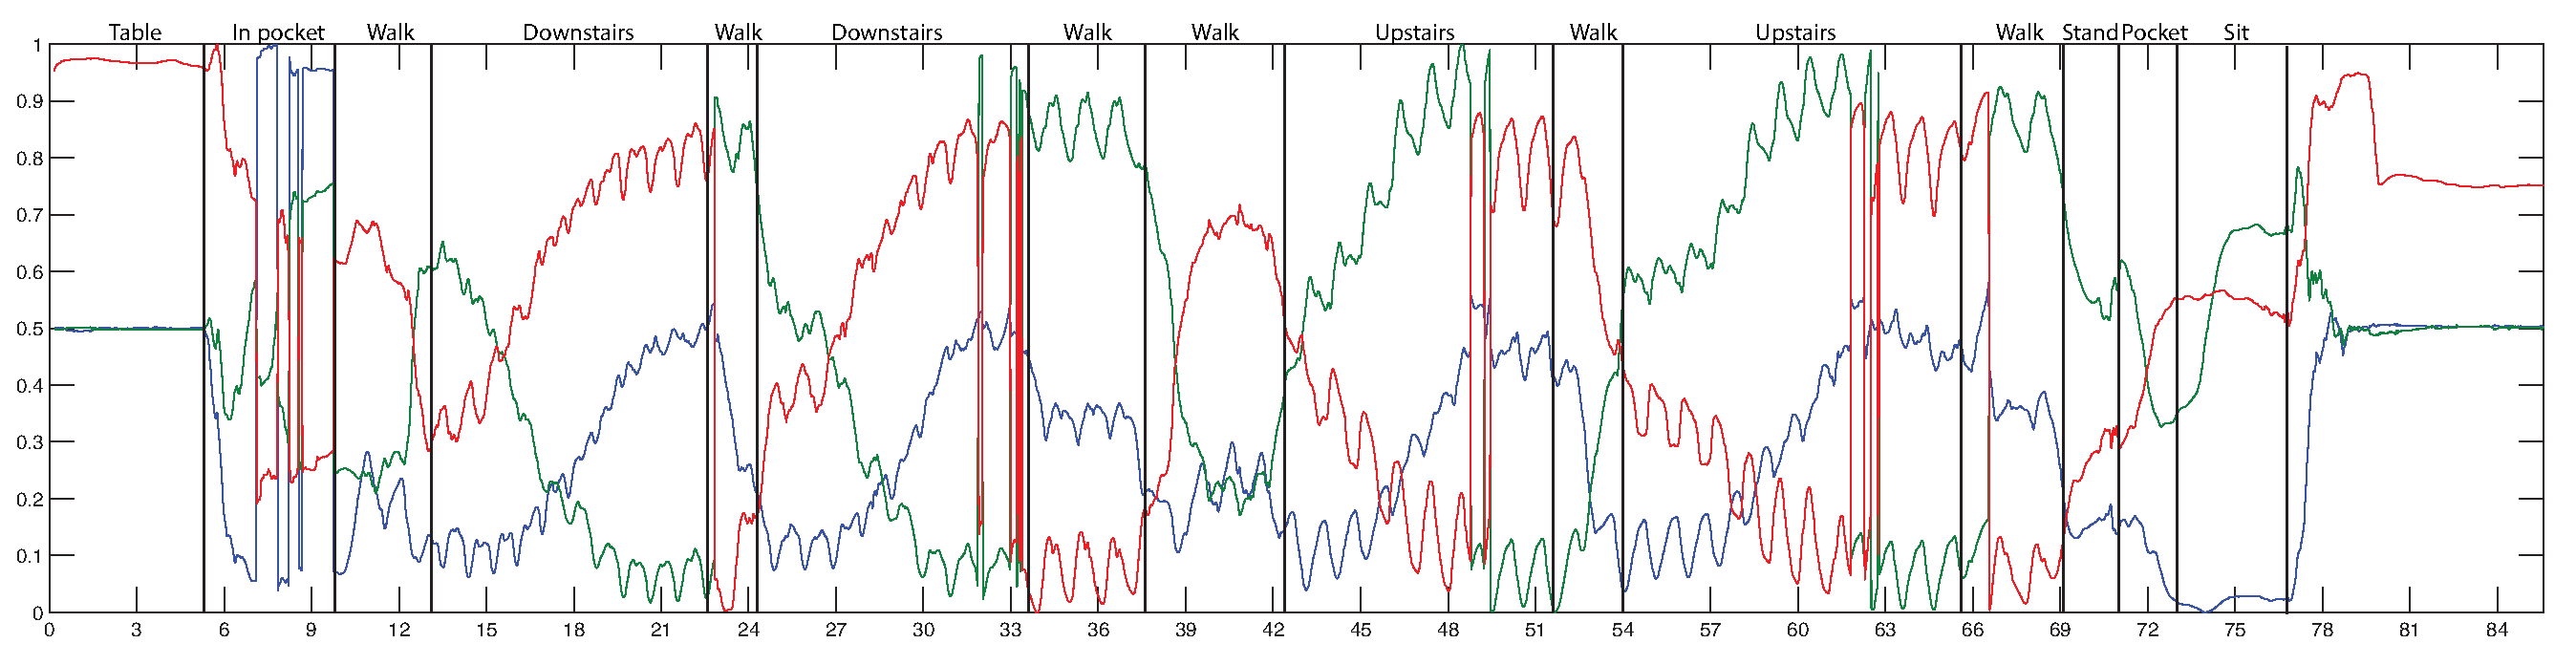
\includegraphics[width=1\textwidth]{./Figures/chapter6/data_collection/stairs-1-marc/data_plot_rot_annotated.eps}
  \caption[R3: rotation]{Run 3: Indoor stairs Marc, rotation}
  \label{fig:data_gathering_run_3_rot}
\end{figure}

\begin{figure}
\centering
  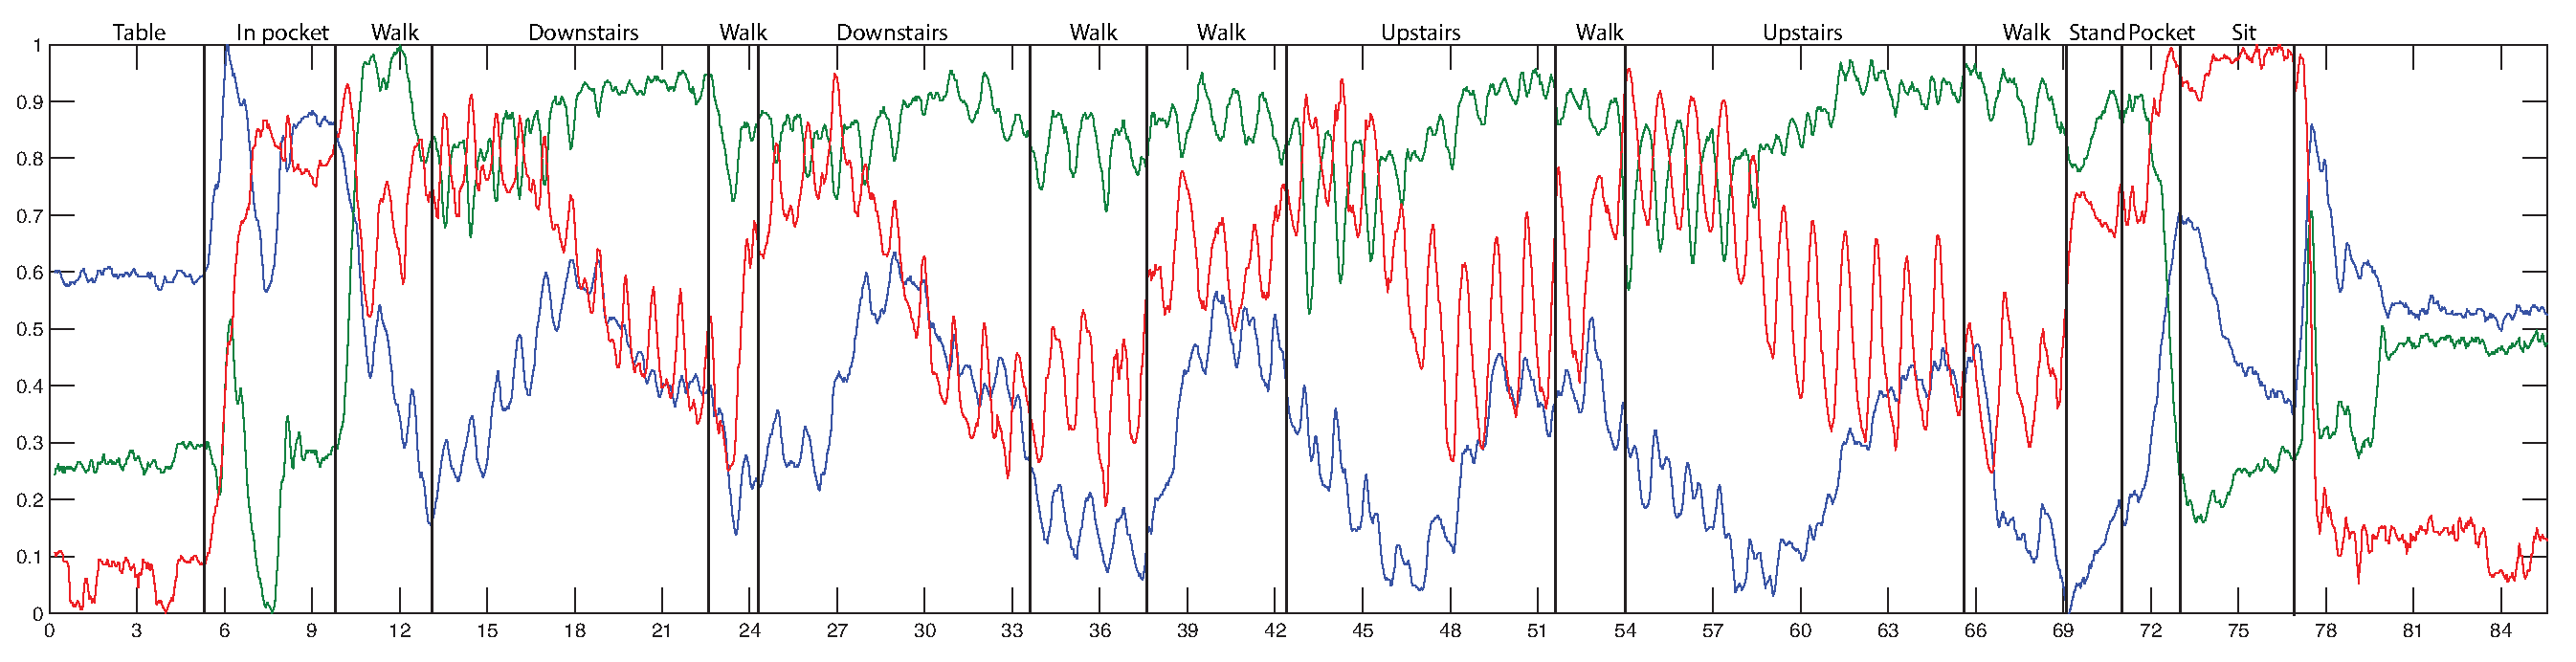
\includegraphics[width=1\textwidth]{./Figures/chapter6/data_collection/stairs-1-marc/data_plot_mag_annotated.eps}
  \caption[R3: mag]{Run 3: Indoor stairs Marc, Mag}
  \label{fig:data_gathering_run_3_mag}
\end{figure}

\begin{figure}
\centering
  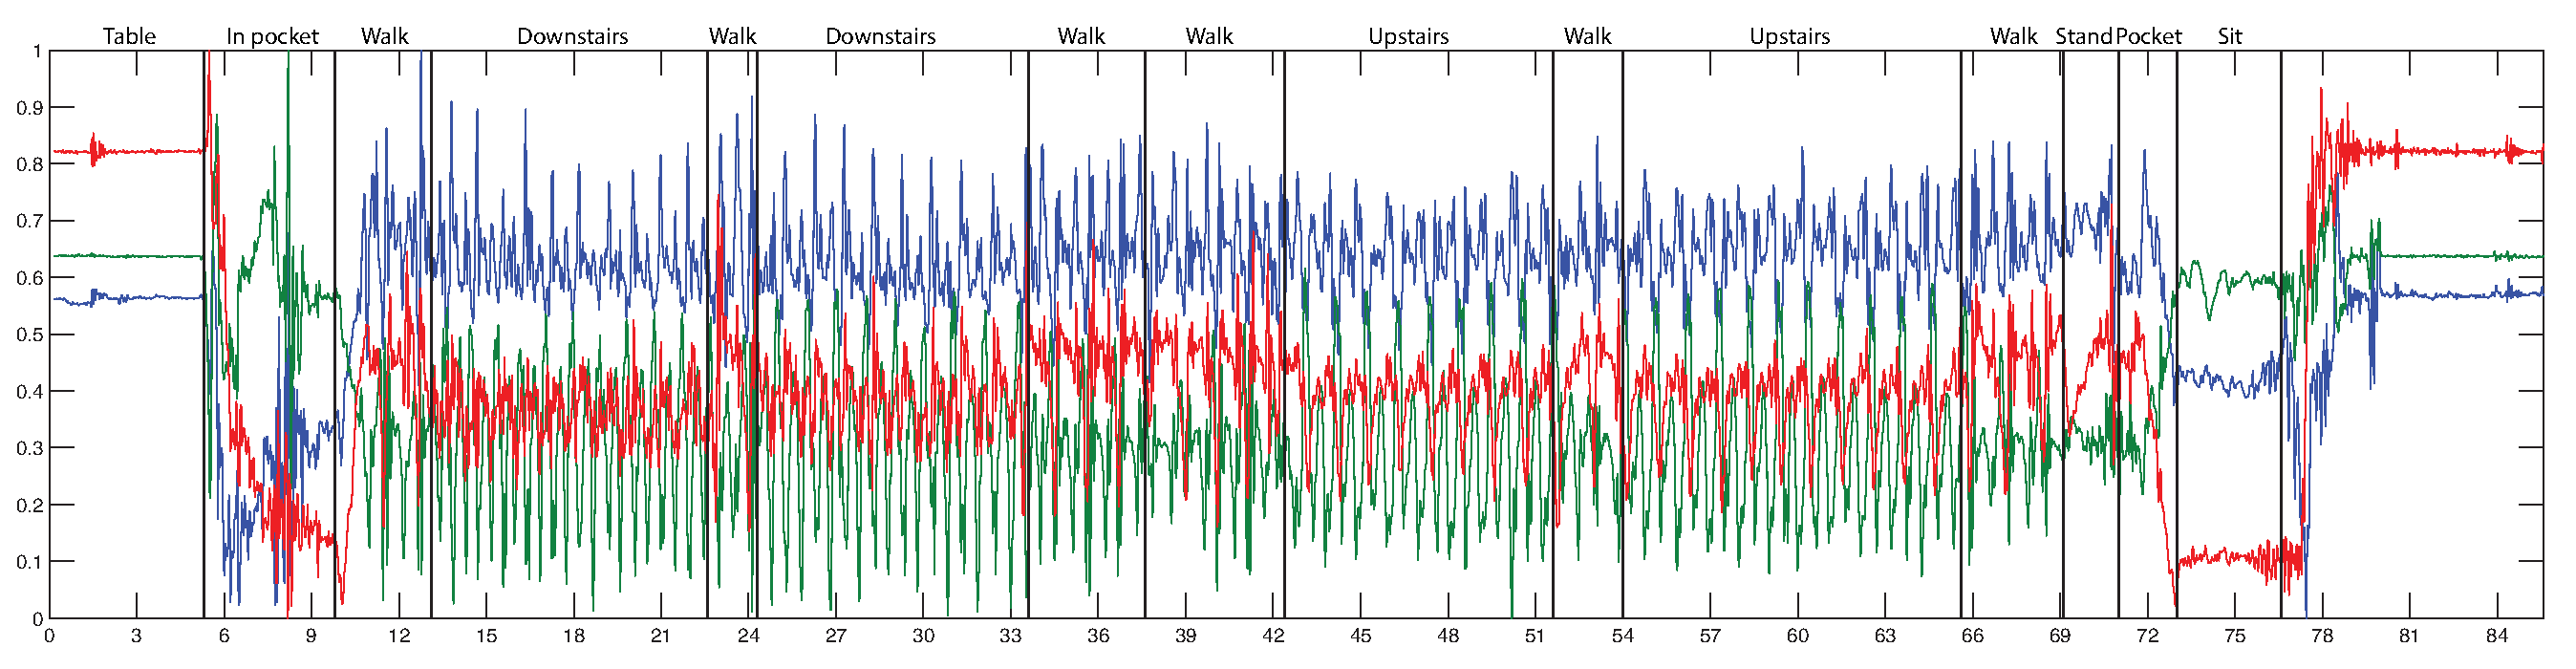
\includegraphics[width=1\textwidth]{./Figures/chapter6/data_collection/stairs-1-marc/data_plot_acc_annotated.eps}
  \caption[R3: accelerometer]{Run 3: Indoor stairs Marc, accelerometer}
  \label{fig:data_gathering_run_3_acc}
\end{figure}


\begin{figure}
\centering
  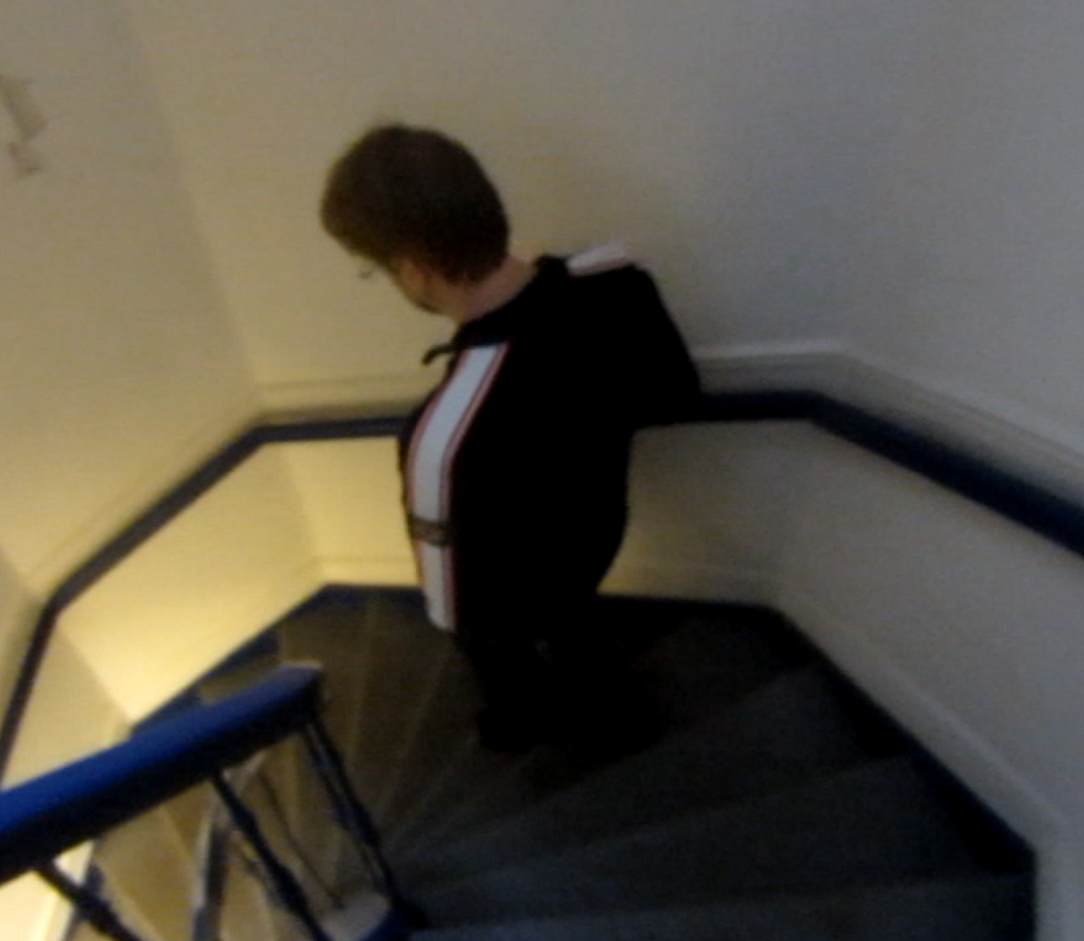
\includegraphics[width=1\textwidth]{./Figures/chapter6/data_collection/stills/marc_downstairs.png}
  \caption[Recording still 8]{Subject 3 descencing the stairs.}
  \label{fig:data_gathering_still_3_descending}
\end{figure}

\begin{figure}
\centering
  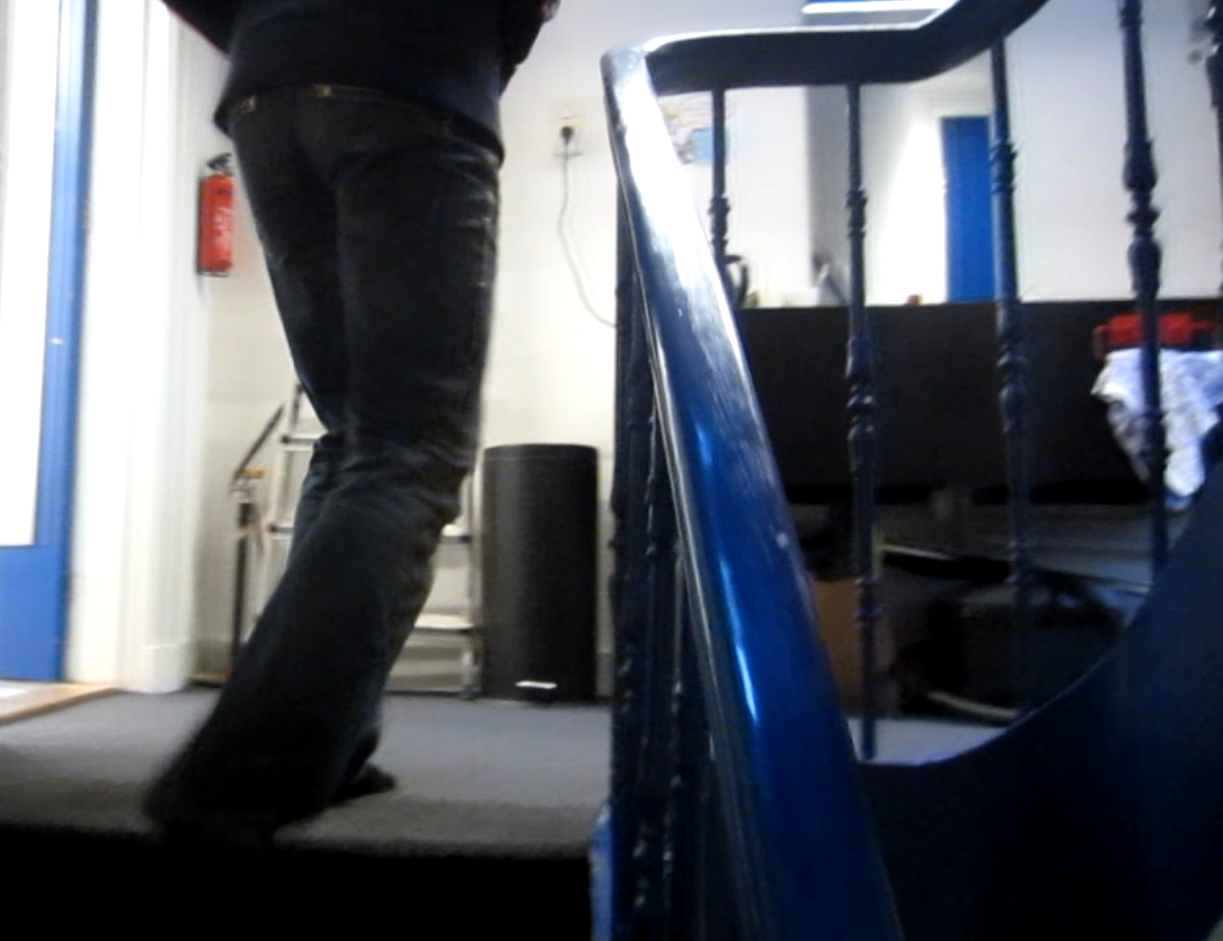
\includegraphics[width=1\textwidth]{./Figures/chapter6/data_collection/stills/marc_stairs_up_walk.png}
  \caption[Recording still 9]{Subject 3 will start walking for a small fragment and will continue ascending the stairs.}
  \label{fig:data_gathering_still_3_ascending}
\end{figure}

\begin{figure}
\centering
  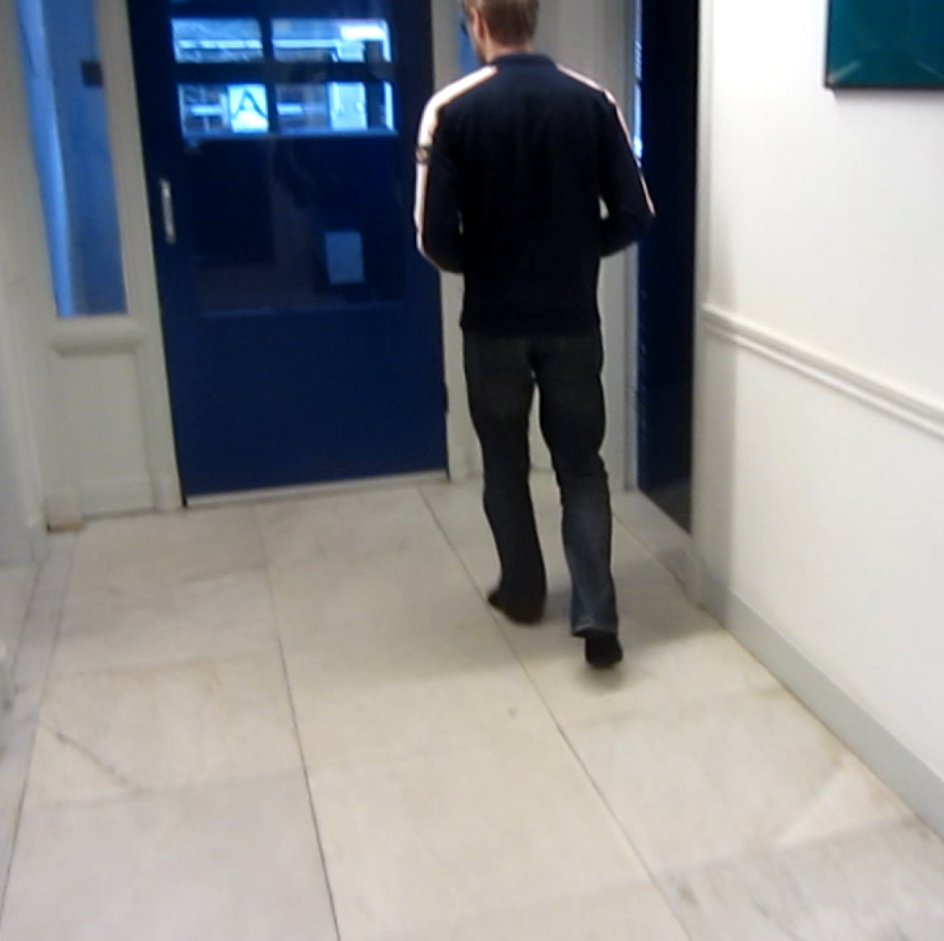
\includegraphics[width=1\textwidth]{./Figures/chapter6/data_collection/stills/marc_walk.png}
  \caption[Recording still 10]{Subject 3 walking in the hallway. He will turn $180^{\circ}$ counter-clockwise.}
  \label{fig:data_gathering_still_3_walk}
\end{figure}